\documentclass[ejs,preprint]{imsart}

% will be filled by editor:
\doi{10.1214/154957804100000000}
\pubyear{0000}
\volume{0}
\firstpage{0}
\lastpage{0}
%\arxiv{}

%\usepackage{color}
\usepackage{amsthm,amsmath,amssymb}
\usepackage{graphicx}
%\usepackage{graphicx}
%\usepackage{esint}
\usepackage{bm}

\newtheorem{definition}{Definition}
\newtheorem{proposition}{Proposition}
\newtheorem{theorem}{Theorem}

\newcommand\E{\mathbb{E}}
%\newcommand\Pr{\mathbb{P}}

\newcommand\cbayes{C^{\mathrm{Bayes}}}
\newcommand\crpnhat{\hat{C}_{n}^{\mathrm{RP}}}
\newcommand\crpnhatstar{\hat{C}_{n}^{\mathrm{RP*}}}
\newcommand\risk{\mathcal{L}}
\newcommand\rrisk{\mathcal{R}}
\newcommand\cabayes{C^{A-\mathrm{Bayes}}}
\newcommand\rabayes{\rrisk^{A-\mathrm{Bayes}}}

\begin{document}

\begin{frontmatter}

% "Title of the Paper"
\title{Axis-Aligned RPE Classification \& Bayesian Random Projection Optimization}
\runtitle{Axis-Aligned RPE \& Bayesian RP Optimization}

% indicate corresponding author with \corref{}
% \author{\fnms{John} \snm{Smith}\thanksref{t2}\corref{}\ead[label=e1]{smith@foo.com}\ead[label=e2,url]{www.foo.com}}
% \thankstext{t2}{Thanks to somebody} 
% \address{line 1\\ line 2\\ \printead{e1}\\ \printead{e2}}

\author{\fnms{Benjamin J.} \snm{Li}\thanksref{t1}\ead[label=e1]{jiachengli@college.harvard.edu}}
\address{Department of Mathematics\\
Harvard University\\
\printead{e1}}
\and
\author{\fnms{Timothy I.} \snm{Cannings}\ead[label=e2]{t.cannings@statlab.cam.ac.uk}}
\address{Statistical Laboratory\\
University of Cambridge\\
\printead{e2}}

\thankstext{t1}{Thanks to my summer research advisor Richard J. Samworth at the Statistical Laboratory, University of Cambridge, under whom this research was performed.} 

\runauthor{B. J. Li and T. I. Cannings}

%\begin{abstract}
%\end{abstract}

%\begin{keyword}[class=MSC]
%\kwd[Primary ]{}
%\kwd{}
%\kwd[; secondary ]{}
%\end{keyword}

%\begin{keyword}
%\kwd{}
%\kwd{}
%\end{keyword}

% history:
% \received{\smonth{1} \syear{0000}}

%\tableofcontents

\end{frontmatter}











\section{Background}

\subsection{Motivation}

A supervised classification problem requires prediction of class labels $Y$ from covariates $X$ given training data. Increasingly often, classification problems are high-dimensional: specifically, the dimension of the feature vectors $p$ is greater than the length of the training set $n$. This violates assumptions in many classification methods, causing poor performance or failure (as in linear discriminant analysis, where the sample covariance matrix when $p\geq n$ is not invertible). Current methods tailored to this situation make strong linearity, sparsity, and/or independence assumptions, as surveyed in \cite{CS15}.

This limits their expressivity, in exchange for statistical power on problems that do fit the assumptions. Ensembling, as used for instance in random forests \cite{Breiman01}, is able to expand expressivity. In that example bootstrap aggregation (bagging), in which the votes of component classifiers trained on bootstrapped data are aggregated, enables the algorithm to express nonlinear decision boundaries even with linear base classifiers.

But bagging is unhelpful in high-dimensional classification -- instead of training component classifiers on ``row-sampled'' data (which effectively reduces $n$), it would be nice to train them on ``column-sampled'' data (reducing $p$).

This motivation is especially strong because we have a powerful guarantee on this ``column-sampling.'' The Johnson-Lindenstrauss Lemma \cite{DG03} states that for any $\epsilon\in(0,1)$ there is some projection $A$ to $\mathbb R^d$ where $d>\frac{8\log n}{\epsilon^2}$ \footnote{Note that this is independent of $p$.} that preserves squared pairwise distances between data points within $\epsilon$, and in fact this matrix can be found stochastically in polynomial time.

We would then be able to perform fairly accurate approximate classification in $\mathbb R^d$. If we aggregate over many classifications on such projected spaces, the idea is that we would have a very accurate consensus estimate, just as bootstrapping obtains via row subsampling.


\subsection{Introduction}

Random projection ensemble (RPE) classification is a very recent method developed to solve the problem of high-dimensional classification.
The fundamental idea is that we can improve the expressiveness and power of any base classifier $\hat C$ under a sufficient dimensionality reduction assumption by applying $\hat C$ to lower-dimensional projections of the feature vectors $A_i X$ and aggregating their responses.

The specifics of the methodology discussed in \cite{CS15} involve drawing $B_{1}\times B_{2}$ $d$-dimensional projections from Haar measure on the space of all such projection matrices, running the base classifier with each of these projections, and then choosing the best of every $B_{2}$ projections, giving a final ensemble of $B_{1}$ projections.

In this paper, we detail two separate improvements, corresponding exactly to the two separate halves of the bound on excess risk in \cite{CS15}. (Below we use notation which we will go over in Sections~\ref{sec:glossary} and \ref{sec:review}).

\subsubsection{First half}

In the first half (Theorem 1 of \cite{CS15}), no distribution on the $B_1$ matrices $\{A_i\}$ is assumed, and it is shown that
\begin{equation}
\risk(\crpnhat) - \risk(\crpnhatstar) \leq O\left(\frac{1}{B_1}\right)
\label{eqn:first-half}
\end{equation}
asymptotically in $B_1$. This is a bound on the difference in risk from only having $B_1$ projections, rather than infinitely many.

As the dimension $p$ of the original data goes up, the space of projections $\mathbb{R}^p\to\mathbb{R}^d$ grows exponentially. It makes some sense to restrict the set of projections on $A$ to be axis-aligned in order to restrict this space. An axis-aligned projection simply picks $d$ basis vectors and drops the rest, bounding the set to $\binom{p}{d}\leq p^{d}/d!$ which is polynomial in $d$.

It turns out that restricting projections to the axis-aligned subspace causes the bound in Equation~\ref{eqn:first-half} to become exponential in $B_1$, and for the bound to hold non-asymptotically under certain conditions!

\subsubsection{Second half}

In the second half (Theorem 2, Proposition 3, and Theorem 5 of \cite{CS15}), the best-of-$B_2$ algorithm is assumed and it is shown that with the $A_i$ chosen by this algorithm, 
\begin{align*}
\risk(\crpnhatstar) - \rrisk(\cbayes)
	&\leq \frac1{\alpha(1-\alpha)}\big[
			\E(\risk_n^{A_1})-\rrisk(\cbayes)
		\big] \qquad\text{(Theorem 2)} \\
	&\leq \frac1{\alpha(1-\alpha)}\big[
			\hat{L}_n^* - \rrisk(\cbayes) + \epsilon_n \\
	&\quad	+ \text{terms from Assumption (A.2)}
		\big] \qquad\text{(Proposition 3)} \\
	&\leq \frac1{\alpha(1-\alpha)}\big[
			(\risk_n^{A^*} - \rrisk^{A^*-\mathrm{Bayes}}) \\
	&\quad	+ (\epsilon_n - \epsilon_n^{A^*}) \\
	&\quad	+ \text{terms from Assumption (A.2)}
		\big] \qquad\text{(Theorem 5)}
\end{align*}
The sum of this with the first-half inequality is then the desired bound on the excess risk of $\crpnhat$.

Choosing the $A_i$ by best-of-$B_2$ reuses no previous information. An avenue for improvement, then, might be to find an algorithm that does reuse previous information.

We propose Bayesian Random Projection Optimization as an elegant way to derive good projection matrices by sampling them from the posterior distribution of $A^*$, the true sufficient dimension reduction matrix from Assumption (A.3). We give a Metropolis-Hastings algorithm for this, and prove a new second-half bound.

\subsection{Glossary}\label{sec:glossary}
\begin{definition}
The \textbf{risk} of a classifier is defined as the \textbf{misclassification
rate} 
\[
\rrisk(C):=\mathbb{P}\left\{ C(X)\neq Y\right\} 
\]
When $C$ is based on data, we write $\hat{C}$ and use the letter
$\risk$ instead of $\rrisk$ to denote risk. The \textbf{excess risk}
of $\hat{C}$ is defined by $\risk(\hat{C})-\rrisk(C^{\mathrm{Bayes}})$.
\end{definition}
There are analogous definitions for estimates of risk based on the
training data:
\begin{definition}
The \textbf{test risk} of a classifier (which I will sometimes refer
to as the \textbf{risk estimate}) replaces $\risk$ with some estimator
of risk based on the data $\hat{L}$, and the \textbf{excess test
risk} (or \textbf{excess risk estimate}) is similarly $\hat{L}(\hat{\theta})-\rrisk(\hat{\theta}^{\mathrm{Bayes}})$.
\end{definition}
Finally, central to the first-half bound, we define the projection matrix space,
and the distribution on it:
\begin{definition}
$\mathcal{A}$ is the subset of $d$-projection matrices that we draw
our random projections from. A random matrix $A$ is a matrix-valued
random variable with some distribution on $\mathcal{A}$.
\end{definition}

There are also some abbreviations we will use throughout the paper:
\begin{itemize}
\item RPE - random projection ensemble (classification)
\item RPE-H - RPE with matrices drawn from Haar measure
\item RPE-A - RPE with uniformly drawn axis-aligned matrices
\end{itemize}

\subsection{Review of RPE theory}\label{sec:review}

The original method made three assumptions in order to deduce that
excess risk $\risk(\crpnhat)-\rrisk(\cbayes)$ is bounded by a sum
of expressions that do not depend on $p$. They are, in order and
paraphrased:\\


\noindent \textbf{Assumption (A.1).} $G_{n,1}$ and $G_{n,2}$ have
second derivatives at the voting threshold $\alpha$, where, given
the true joint distribution of the training data $(X,Y)$, $G_{n,i}$
is the CDF of the probability that the base classifier $\hat{C}_{n}$
will classify a random projection of $X$ as class $i$.\\


This assumption is used to show that the risk of the finite
RPE classifier $\crpnhat$ (with choices of base classifier $\hat{C}_{n}$,
voting threshold $\alpha$, and finite ensemble size parameters $B_{1}$
and $B_{2}$) is well-approximated by that of the infinite-simulation
RPE classifier $\crpnhatstar$ (with the same choices of $\hat{C}_{n}$
and $\alpha$). This result is \textbf{Theorem 1}, and does not involve
the distribution on the projection matrices $A_{i}$ other than that
they are independent and identically distributed, and independent
of $(X,Y)$. This concludes the first-half bound.\\


\textbf{Theorem 2}, bounding $\risk(\crpnhatstar)-\rrisk(\cbayes)$,
does not involve the distribution on the projection matrices $A_{i}$
other than that they are independent and identically distributed,
and independent of $(X,Y)$. Thus, this result pulls smoothly into
the axis-aligned case.


The next assumption involves the production of a good selection of random projections by taking the best projection in each row from a $B_{1}\times B_{2}$-sized grid of i.i.d. random projections from some base distribution (Haar measure as generally discussed in the original paper). To make conclusions about the test error, we define $\beta_{n}(j)$ as the discrete CDF of $n\left(\hat{L}_{n}^{A}-\hat{L}_{n}^{*}\right)$ (which is the random variable $n\hat{L}_{n}^{A}=\sum_{(x,y)}I(\hat{C}_{n}^{A}(x)\neq y)$ minus a constant, where $A$ is random).\\


\noindent \textbf{Assumption (A.2).} There is some $B_{0}\in(0,1)$
and $\beta,\rho>0$ such that the histogram $\beta_{n}(j)$ is bounded
below by the discrete CDF $\beta_{0}+\frac{\beta j^{\rho}}{n^{\rho}}$
for all $j$ below $n\left(\frac{\log^{2}B_{2}}{\beta B_{2}}\right)^{1/\rho}+1$.
It is particularly noted that as $B_{2}$ goes up, the strength of
the condition decreases (a smaller bit of the left side of the CDF
is constrained).\\


From this, \textbf{Proposition 3} bounds the expected excess risk
$\mathbb{E}(\risk_{n}^{A_{1}})-\rrisk(\cbayes)$ of a best-of-$B_{2}$
projection by an expression involving $\hat{L}_{n}^{*}-\rrisk(\cbayes)$,
the minimum excess risk estimate over all $A\in\mathcal A$. Intuitively,
we expect this to be small when the Bayes classifier indeed only takes
into account $d$ of the dimensions, which leads to the following
definition and assumption:

\begin{definition}
Let $\cabayes$ be the \textbf{projected Bayes classifier}, defined
as the Bayes classifier on the joint distribution $(AX,Y)$, and $\rabayes$
its risk.
\end{definition}


\noindent \textbf{Assumption (A.3).} There is some projection $A^{*}\in\mathcal{A}$
such that the Bayes classifier and the projected Bayes classifier
are the same except on a set of measure zero.\\


\textbf{Proposition 4} goes to show that (A.3) holds under the sufficient
dimension reduction condition (there exists a dimension reduction
$R$ such that $R(X)$ is sufficient, ie. $Y\,|\,R(X)$ has the same
distribution as $Y\,|\,X$). Naturally one would expect that if (A.3)
holds, $\hat{L}_{n}^{*}$ would be close to $\rrisk(\cbayes)$, which
is quantified in \textbf{Theorem 5}.





















\section{Axis-aligned RPE theory}

\subsection{Effect of axis-alignment on $G_{n,i}$ curves}

\begin{figure}
\begin{centering}
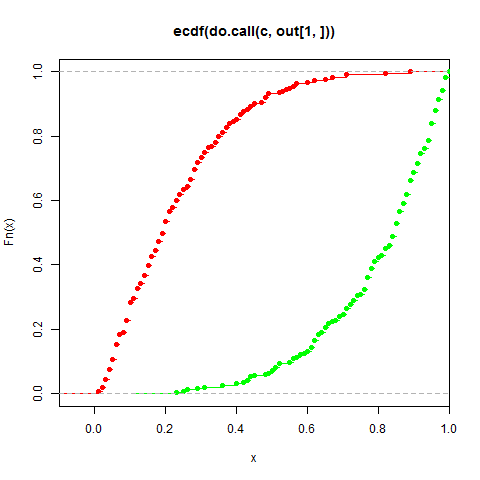
\includegraphics[scale=0.35]{G_ni}%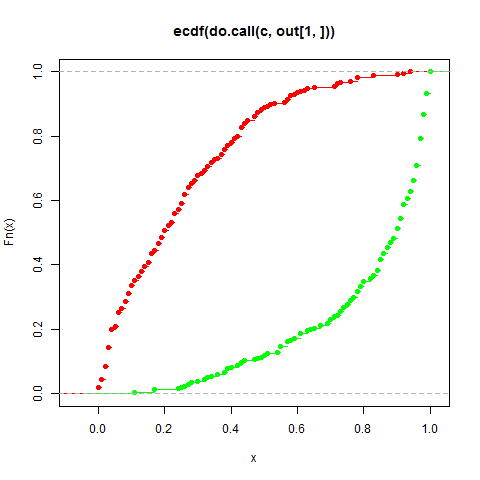
\includegraphics[scale=0.35]{G_ni_axis}
\par\end{centering}

\caption{The empirical $G_{n,i}$ curves for standard runs
of Model 1 in \cite{CS15} ($n_{\mathrm{train}}=50$ and $B_{1}=B_{2}=100$) with RPE-H LDA,
% (left) versus RPE-A LDA (right),
averaged over 10 instances.}

\label{fig:std-run-g-curves}
\end{figure}


Central to Theorem 1, the most involved theoretical result in the paper, are
the $G_{n,i}$ curves. They are estimated and plotted in Figure~\ref{fig:std-run-g-curves}
for a standard run of Model 1 with both RPE-H LDA and RPE-A LDA. (Note
that adjusting $n_{\mathrm{train}}$ changes the shape of these curves,
which is why they've been averaged over 10 instances instead of simply
run on 10 times more data.)

What effect would imposing axis-alignment have on these centrally-important curves? Finite $\mathcal{A}$ implies a discrete distribution on $A$, which means that the $G_{n,i}$
are step functions -- a much stronger assumption than second-differentiability
at the voting threshold $\alpha$!

%\begin{figure}
%\begin{centering}
%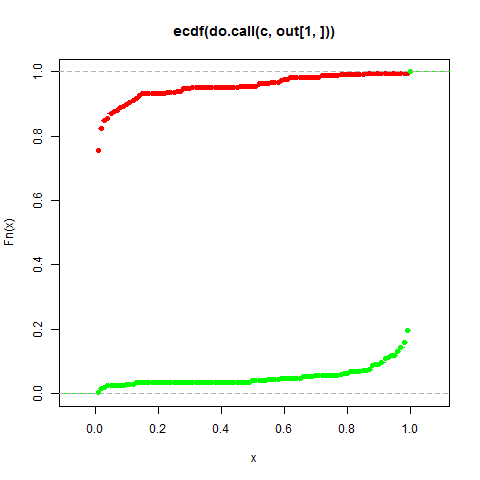
\includegraphics[scale=0.35]{G_ni_mini}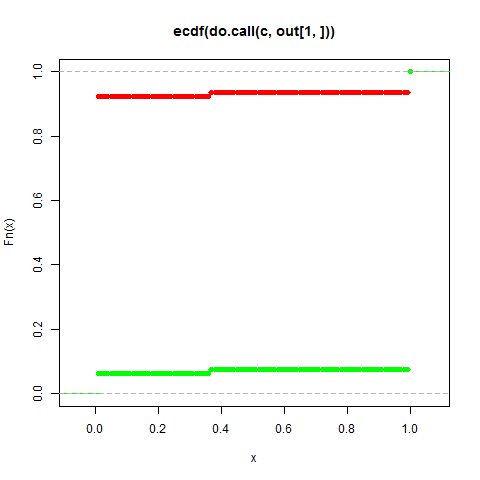
\includegraphics[scale=0.35]{G_ni_mini_axis}
%\par\end{centering}
%
%\caption{The empirical $G_{n,i}$ curves for $p=5$
%and $d=2$, again with RPE-H LDA (left) and RPE-A LDA (right), averaged
%over 10 instances. The difference is much clearer.}
%
%
%\label{fig:mini-run-g-curves}
%\end{figure}
%
%
%As a much clearer illustration, Figure~\ref{fig:mini-run-g-curves} shows
%these curves with $p=5$ and $d=2$.

\subsection{Effect of axis-alignment on second-half bound}

Restricting $\mathcal A$ to axis-aligned projections does not affect Theorem 2, which is independent of the distribution of $A$.

The CDF $\beta_{n}(j)$ can still be defined, where $A$ is now distributed
uniformly on the set of axis-aligned projection matrices, so Assumption
(A.2) and Proposition 3 can remain unchanged (where $A_{1}$ is now
a best-of-$B_{2}$ axis-aligned projection matrix).

Assumption (A.3) has a simple modification (compatible with Proposition
4) to make Theorem 5 hold for axis-aligned projections:\\


\noindent \textbf{Assumption (A.3').} There is some \emph{axis-aligned}
projection $A^{*}\in\mathcal{A}$ such that the Bayes classifier and
the projected Bayes classifier are the same except on a set of measure
zero.\\


Thus, all that's left to fill in are the new (A.1) and Theorem 1 (and
replacing the Theorem 1-derived part in Theorem 5's bound with the
corresponding new and improved expression).


\subsection{New theorem}

We revise Assumption (A.1):\\

\noindent \textbf{Assumption (A.1$'$).} $G_{n,1}$ and $G_{n,2}$ are
constant in a neighborhood of $\alpha$.\\

It is easy to show that this assumption holds for our axis-aligned
case.

\begin{proposition}
Allowing infinitesimal perturbation of $\alpha$,\footnote{Practically, we would choose $\alpha$ with its distance to an element of $R$ in mind, as we discuss later, so this is somewhat irrelevant.} Assumption (A.1$'$) holds for $\mathcal{A}$ as the set of axis-aligned
$d\times p$ projections (or any subset thereof) and $A$ a matrix-valued
random variable with this set as its support, with some distribution\footnote{For example, uniform over $\mathcal{A}$, or as is done in the package,
chosen from the best of $B_{2}$ uniform candidates.} given by probabilities $q_{B}$ for all $B\in\mathcal{A}$.
\end{proposition}


\begin{proof}
We have that 
\begin{eqnarray*}
G_{n,1}(\alpha) & = & \mathbb{P}\left\{ \mathbb{P}\left\{ \hat{C}_{n}^{A}(X)=1\,\Big|\,X\right\} \leq\alpha\,\Big|\,Y=1\right\} \\
 & = & \mathbb{P}\left\{ \sum_{B\in\mathcal{A}}q_{B}I\left\{ \hat{C}_{n}^{B}(X)=1\right\} \leq\alpha\,\Big|\,Y=1\right\} 
\end{eqnarray*}
 is the CDF of a finite weighted sum of indicators. It can be seen
as a step function with up to $||\mathcal{A}||$ jumps; let the set of the
horizontal locations of these jumps be $R_{1}$ and let the corresponding
vertical heights be $s_{r}$ (ie. such that $\sum_{r\in R_{1}}s_{r}=1$).
Note that $R_{1}$ has Lebesgue measure zero inside $[0,1]$ and $G_{n,1}$
is flat (thus has zero first and second derivatives) outside of $R_{1}$.

The same holds for $G_{n,2}$; let the horizontal locations of its
jumps be $R_{2}$ and the vertical heights be $t_{r}$ analogously.

Then outside of the set $R=R_{1}\cup R_{2}$, $G_{n,1}$ and $G_{n,2}$ are locally constant. If we allow infinitesimal perturbation of $\alpha$, it will never fall into this set.
\end{proof}


Note that the set $R$ has cardinality at most $2||\mathcal{A}||=2\binom{p}{d}\leq2\frac{p^{d}}{d!}$.\\


Now we design an analogous version of Theorem 1:\\


\noindent \textbf{Theorem 1$'$.} \emph{Assume (A.1$'$). Then 
\[
\risk\left(\crpnhat\right)-\risk\left(\crpnhatstar\right)=o\left(B_{1}^{-M}\right)
\]
 as $B_{1}\to\infty$ for all $M\in\mathbb{N}$.}\footnote{\noindent Note that here $\crpnhatstar$ represents the infinite axis-aligned
projection RPE classifier, so that although this bound is tighter,
the infinite projection classifier we're approximating may be farther
from the Bayes classifier than the general case. But this doesn't affect our theory, as
we modified (A.3) so that $A^{*}$ must be axis-aligned.}

\emph{Moreover, there exists some $C>0$ such that for all $B_1\geq C$, the non-asymptotic bound
\[
\risk\left(\crpnhat\right)-\risk\left(\crpnhatstar\right)=e^{-2\log^2 B_1}
\]
holds.}


\begin{proof}
As before we have 
\begin{eqnarray*}
\risk(\crpnhat) & = & \pi_{1}\mathbb{P}\left\{ \crpnhat(X)=2\,|\,Y=1\right\} +\pi_{2}\mathbb{P}\left\{ \crpnhat(X)=1\,|\,Y=2\right\} \\
 & = & \pi_{1}\mathbb{P}\left\{ \hat{\nu}_{n}^{B_{1}}(X)<\alpha\,|\,Y=1\right\} +\pi_{2}\mathbb{P}\left\{ \hat{\nu}_{n}^{B_{1}}(X)\geq\alpha\,|\,Y=2\right\} 
\end{eqnarray*}
 where $\hat{\nu}_{n}^{B_{1}}(x):=\frac{1}{B_{1}}\sum_{b_{1}=1}^{B_{1}}I\left\{ \hat{C}_{n}^{A_{b_{1}}}(x)=1\right\} $.
Conditional on the mean $\hat{\mu}_{n}(X)=\theta$ of the $I\left\{ \hat{C}_{n}^{A_{b_{1}}}(x)=1\right\} $,
they are i.i.d. $\mathrm{Bern}(\theta)$. As $G_{n,1}$ is the CDF
of $\hat{\mu}_{n}(X)\,|\,\{Y=1\}$, we can write 
\begin{eqnarray*}
\mathbb{P}\left\{ \hat{\nu}_{n}^{B_{1}}(X)<\alpha\,|\,Y=1\right\}  & = & \int_{0}^{1}\!\mathbb{P}\left\{ \frac{1}{B_{1}}\sum_{b_{1}=1}^{B_{1}}I\left\{ \hat{C}_{n}^{A_{b_{1}}}(x)=1\right\} <\alpha\,\bigg|\,\hat{\mu}_{n}(X)=\theta\right\} \,dG_{n,1}(\theta)\\
 & = & \int_{0}^{1}\!\mathbb{P}(T<B_{1}\alpha)\,dG_{n,1}(\theta)
\end{eqnarray*}
 for $T\sim\mathrm{Bin}(B_{1},\theta)$. Combining with the similar
result for $G_{n,2}$ gives 
\[
\risk(\crpnhat)=\pi_{2}+\int_{0}^{1}\!\mathbb{P}(T<B_{1}\alpha)\,dG_{n}^{\circ}(\theta)
\]
 where $G_{n}^{\circ}=\pi_{1}G_{n,1}-\pi_{2}G_{n,2}$. Subtracting the statement 
\[
\risk\left(\crpnhatstar\right)=\pi_{1}G_{n,1}(\alpha)+\pi_{2}\left(1-G_{n,2}(\alpha)\right)
\]
 gives 
\[
\risk\left(\crpnhat\right)-\risk\left(\crpnhatstar\right)=\int_{0}^{1}\!\mathbb{P}(T<B_{1}\alpha)-I\{\theta<\alpha\}\,dG_{n}^{\circ}(\theta)
\]


As before we show that 
\[
\int_{0}^{1}\!\mathbb{P}(T<B_{1}\alpha)-I\{\theta<\alpha\}\,dG_{n}^{\circ}(\theta)=\int_{\alpha-\epsilon}^{\alpha+\epsilon}\!\mathbb{P}(T<B_{1}\alpha)-I\{\theta<\alpha\}\,dG_{n}^{\circ}(\theta)+o(B_{1}^{-M})
\]
 as $B_{1}\to\infty$ for all $M\in\mathbb{N}$, by Hoeffding's inequality:
for $\epsilon=\frac{\log B_{1}}{\sqrt{B_{1}}}$ and all $M$ we have
\[
\sup_{|\theta-\alpha|\geq\epsilon}\left|\mathbb{P}(T<B_{1}\alpha)-I\{\theta<\alpha\}\right|\leq\sup_{|\theta-\alpha|\geq\epsilon}\exp\left\{ -2B_{1}(\theta-\alpha)^{2}\right\} \leq e^{-2\log^{2}B_{1}}=o(B_{1}^{-M})
\]


Let $I=(\alpha-\epsilon,\alpha+\epsilon)$. Note that $G_{n,1}$ is
the CDF of a discrete random variable with values $r\in R_{1}$ and
probabilities $s_{r}$, and $G_{n,2}$ the same for $t_r$, so that 
\begin{eqnarray*}
\int_{\alpha-\epsilon}^{\alpha+\epsilon}\!\mathbb{P}(T<B_{1}\alpha)-I\{\theta<\alpha\}\,dG_{n}^{\circ}(\theta) & = & \pi_{1}\sum_{r\in R_{1}\cap I}s_{r}\left(\mathbb{P}(T<B_{1}\alpha)-I\{r<\alpha\}\right)\\
 &  & -\pi_{2}\sum_{r\in R_{2}\cap I}t_{r}\left(\mathbb{P}(T<B_{1}\alpha)-I\{r<\alpha\}\right)
\end{eqnarray*}


This leads to the conclusion: we can make both $R_{1}\cap I$
and $R_{2}\cap I$ empty by setting $B_{1}$ high enough that $\epsilon<\min_{r\in R_{1}\cup R_{2}}|\alpha-r|$.
\end{proof}

In other words, one can get bounds exponentially close to $\crpnhatstar$
(the infinite axis-aligned projection classifier), as opposed to only
linearly close to the general infinite projection classifier.

As $\epsilon=\frac{\log B_{1}}{\sqrt{B_{1}}}$ is strictly decreasing in $B_{1}$ for all $B_{1}>1$, and has inverse $B_{1}=\exp\left(-2W_{-1}(-\frac{\epsilon}{2})\right)$ involving the Lambert $W$ function \cite{CGHJK96}, this exponential behavior kicks in non-asymptotically at
\[
B_{1}>\exp\left(-2W_{-1}\left(-\frac{\min|\alpha-r|}{2}\right)\right).
\]

\subsection{Estimating $\min|\alpha-r|$}

In the process of determining this lower bound, an issue arises with the determination of $\min|\alpha-r|$.
We only know $\hat{\pi}_{1}n_{\mathrm{train}}$ elements of $R_{1}$, which is generally not close to the cardinality of $R_{1}$ (which can be as big as $2^{||\mathcal{A}||}=2^{\binom{p}{d}}$).
However, we can estimate $\min|\alpha-r_{1}|$ by the following procedure:
\begin{enumerate}
\item Smooth $\hat{g}_{n,1}$ (by, for instance, taking $\tilde{g}_{n,1}$
as the sum of Gaussians at each known element of $R_{1}$ with some
specified bandwidth).
\item Evaluate this smoothed empirical density at $\alpha$.
\item Note that on average, a $\tilde{g}_{n,1}(\alpha)\times\delta$ slice
of the density will contain $\tilde{g}_{n,1}\delta||R_{1}||$ points;
setting this to 1 gives $\delta=\frac{1}{\tilde{g}_{n,1}(\alpha)\cdot||R_{1}||}$
as our estimate for $\min|\alpha-r_{1}|$.
\end{enumerate}
Combined with previous observations, this means that generally we
need 
\[
B_{1}>\exp\left\{ -2W_{-1}\left(-\frac{1}{2^{\binom{p}{d}+1}\cdot\max_i\tilde{g}_{n,i}(\alpha)}\right)\right\} 
\]
 (where $W_{-1}$, also known as the product logarithm, vanishes
more slowly than the logarithm -- see the next section).

If $\max_i\tilde{g}_{n,i}(\alpha)$ doesn't vanish quickly enough, this
expression will be dominated by the exponential behavior of $||R||$.


\subsection{Discussion \& future work}

\begin{figure}
\begin{centering}
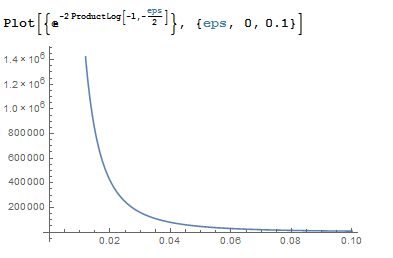
\includegraphics[scale=0.8]{aa-b1-as-func-of-eps.PNG}
\par\end{centering}

\caption{Lower bound for $B_{1}$ as a function of upper bound for $\epsilon$.}

\label{fig:b1-as-func-of-eps}
\end{figure}


Although the theorem is an impressive statement, the lower bound
for $B_{1}$ before the exponential decay of error in Theorem 1$'$ kicks
in is very large and grows extremely quickly in $p$ and $d$, as
a result of the exponential (see Figure~\ref{fig:b1-as-func-of-eps}).
For instance, we need $\max_i g_{n,i}(\alpha)$
at a value of $2^{-\binom{p}{d}+1}$ to put the minimum $B_{1}$ for
exponential behavior at $74.2$.

This theoretical result would go hand-in-hand with a good algorithm for choosing projections. If we have a good method of optimizing projections, then $g_{n,1}$ and $g_{n,2}$ (the density functions from which we draw $r_{1}\in R_{1}$ and $r_{2}\in R_{2}$ respectively -- see Figure~\ref{fig:r1-dist}) would tend to be skewed far left and far right respectively. Optimal values of $\alpha$ would then be in the middle, where $R_{1}\cup R_{2}$ is much less dense, and thus $\min|r-\alpha|$ larger, allowing for exponential behavior with lower $B_{1}$.

\begin{figure}
\begin{centering}
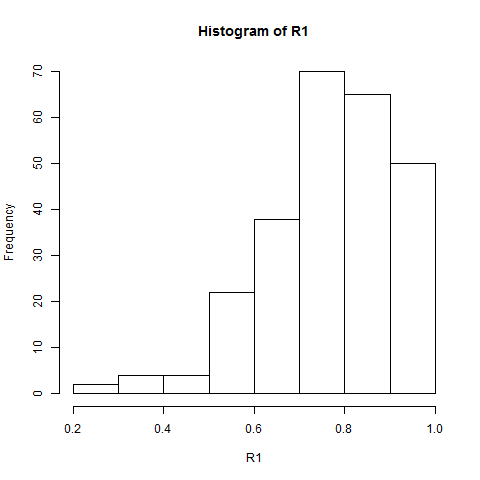
\includegraphics[scale=0.5]{r1_dist}
\par\end{centering}

\caption{$g_{n,1}$ (the distribution of $r_{1}=\mathbb{P}\left(\hat{C}_{n}^{A}(X)=1\,|\,X,Y=1\right)$)
for Model 1 with standard parameters, estimated from 10 runs.}


\label{fig:r1-dist}
\end{figure}

Even more ideally we would have an algorithm for $A_{1}$ that almost never lets $r_{1}$ or $r_{2}\in(\alpha-\epsilon,\alpha+\epsilon)$
-- then $\risk\left(\crpnhat\right)-\risk\left(\crpnhatstar\right)$ would decay exponentially in $B_{1}$ with no minimum bound on $B_{1}$! This would apply even to Haar or other base distributions on projection matrix space.

A simple example would be to have the sampler purposefully reject any such draw of $A_1$ for which $\hat r_i = \frac1n\sum_{j=1}^n I(\hat C_n^{A_1}(X)=1 \,|\, X,Y=i) \in (\alpha+\epsilon, \alpha-\epsilon)$ -- the interval can be widened to compensate for the inaccuracy of $\hat r_i$.


































\section{Bayesian random projection optimization}

The second part of this paper deals with the second-half inequality, bounding $\risk(\crpnhatstar) - \rrisk(\cbayes)$ by more efficiently sampling $B_1$ projections that comprise the ensemble. We make no assumptions about $\mathcal A$, rendering this part independent of (but complementary to) the axis-aligned theory above.

However, Assumption (A.3) plays a crucial part, perhaps moreso than in the original method, in that we use it word-for-word as the core of our Bayesian model. Our model states that there \emph{is} a true $A^*$, and we use it as our model parameter $\theta$.

Ultimately, our goal is to utilize the Bayesian framework to obtain a ``best-possible'' ensemble classifier, in the sense that we've used all information available to us, and the remaining error is irreducible.

\subsection{Bayesian motivation}

Define the following quantities:

\begin{center}
	\begin{tabular}{r|l}
		Parameter & $A^*$ \\
		Data & $D=(X,Y)$ \\
		Model (likelihood) & $f(D\,|\,A^*)$ \\
		Prior & $\tau(A^*)=$ Haar measure on $\mathcal{A}$ \\
		Marginal & $m(D) = \int\!f(D\,|\,A^*)\pi(A^*)\,dA^*$ \\
		Posterior & $\pi(A^*\,|\,D) = \frac{f(D\,|\,A^*)\pi(A^*)}{m(D)}$
	\end{tabular}
\end{center}

\subsubsection{Illustration}

\begin{figure}
\begin{centering}
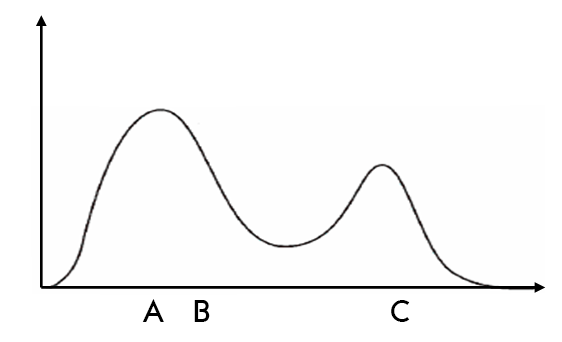
\includegraphics[scale=0.4]{illustration1}
\caption{An example posterior density $\pi(A^*\,|\,\mathrm{data})$, visualized in one dimension.
\label{fig:illust1}}
\par\end{centering}
\end{figure}

In Figure~\ref{fig:illust1}, point (A) would be the single (point) estimate $\widehat{A^*}$ in the original method of drawing the $A_i$ (each one as the projection with the minimum test error or ``highest likelihood'' out of $B_2$ projections drawn from the prior).

However, the distribution itself provides much more information than the point estimate. There is ample probability of finding $A^*$ at (B), slightly off from the mode, or at (C) in an entirely separate probability cluster. In particular for (C), the best-of-$B_2$ method will nearly never draw representatives from the smaller peak. In fact, the chance becomes vanishingly small as $B_2\to\infty$.

\begin{figure}
\begin{centering}
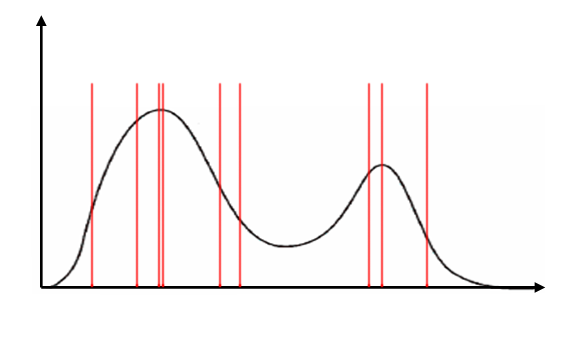
\includegraphics[scale=0.4]{illustration2}
\par\end{centering}
\caption{An ensemble representing (approximating) $\pi(A^*\,|\,\mathrm{data})$.}
\label{fig:illust2}
\end{figure}

\subsubsection{Bootstrap MAP versus density estimation}

For this section think of the likelihood of $A^*$ as the classification accuracy on $A^*X$ by the base classifier. We will give a principled explanation for why this makes sense further on.

In Bayesian terminology, the original method of \cite{CS15} is approximating the MAP (maximum a posteriori) estimate via best-of-$B_2$, and then maintaining some variation in that estimate by repeating this $B_1$ times and ensembling the results. This technique has proven quite effective, and might be referred to as a ``\textbf{bootstrap MAP}'' approach from our Bayesian perspective.

Note that the information from $B_1(B_2-1)$ of the projection matrices drawn goes largely unused. It would be nice to fully utilize the likelihoods calculated for all $B_1B_2$ samples. This is equivalent to saying we should use a full density estimate, not just a series of MAP estimates, in our ensemble method.

\subsection{Bayesian framework}

\subsubsection{Drawing directly from $\pi(A^*\,|\,\mathrm{data})$}

It would be nice to use the full information of the posterior distribution, rather than $B_1$ independent resamples of the single-point MAP estimate. The objectively-best way to do this would be to draw our $B_1$ projection matrices \emph{directly from $\pi(A^*\,|\,\mathrm{data})$}, the posterior density on projection matrix space, as shown in Figure~\ref{fig:illust2}.

The accuracy of an RPE classifier based directly on $\pi(A^*\,|\,\mathrm{data})$ is, in the Bayesian sense, the best possible performance we can get with the assumptions and data we have. As we obtain more data (as $n\to\infty$), $\pi(A^*\,|\,\mathrm{data})$ will approach the true distribution $\pi_0 = \delta_{A^*_\mathrm{true}}$, and the risk will approach the Bayes risk.

Let $g(p)=\E_{A\sim p}(\risk_n^A)$ be a functional taking some distribution of projection matrices $p$ to the expected risk over that distribution. In other words, if we drew infinitely many $A_i$ from $p$, the risk of the resulting RPE classifier would be $g(p)$.

For $n$ fixed, $g(\pi)-g(\pi_0)=\epsilon_\mathrm{irr}$ is the irreducible error in our scenario.

\subsubsection{Drawing from an ergodic Markov chain with stationary distribution $\pi(A^*\,|\,\mathrm{data})$}

Drawing directly from $\pi(A^*\,|\,\mathrm{data})$ is infeasible (it would require computing the partition function $m(D)$ which would take $||\mathcal A||$ evaluations of the base classifier).

However, if we have an ergodic Markov chain with $\pi(A^*\,|\,\mathrm{data})$ as its stationary distribution, there is an powerful result we can invoke from ergodic theory. This theorem can be interpreted as a type of law of large numbers, saying that for an ergodic random process, the time average moves closer to the space average as time goes on.

The textbook \cite{MT93} is a general reference for ergodic theory on Markov chains, while the lecture notes \cite{Sarig08} and \cite{Geyer12} provide a more concise summary. The weak ergodic theorem cited here is Theorem 2.1 (von Neumann's Mean Ergodic Theorem) from \cite{Sarig08}; Theorem 2.2 (Birkhoff's Pointwise Ergodic Theorem) is a stronger result (almost everywhere convergence) that we don't need. The geometric ergodic theorem is given two entire chapters, Chapters 15 \& 16, in \cite{MT93}, and also appears a remark at the end of Section 1.5.4.3 (Proof of the Ergodic Theorem for Markov chains) of \cite{Sarig08}, after the proof.

\begin{theorem}
(Weak ergodic theorem) For any functional $g(p)=\E_{A\sim p}(h(A))$, 
\[
\sum_{i=1}^{B_1}\frac{1}{B_1} h(A_i) \overset{p}{\to} g(\pi)
\]
as $B_1\to\infty$, where the $A_i$ are drawn from an ergodic Markov chain $\bm{\Phi}$ with stationary distribution $\pi$.
\end{theorem}

\begin{theorem}
(Uniform ergodic theorem) If $\bm\Phi$ is uniformly ergodic (satisfying one of the seven equivalent conditions in Theorem 16.0.2 of \cite{MT93}), then for any functional $g(p)=\E_{A\sim p}(h(A))$, 
\[
\left|\sum_{i=1}^{B_1}\frac{1}{B_1} h(A_i)-g(\pi)\right|\leq C\cdot \rho^{B_1}
\]
in probability for some $\rho<1$, independent of the initial state.
\end{theorem}

\{There is also a geometric ergodic theorem, which is weaker than uniform ergodicity. However, uniform ergodicity would be ideal.\}

Ergodicity is implied by irreducibility, aperiodicity, and positive recurrence, which Metropolis-Hastings algorithms satisfy (this is the type of inference algorithm we will apply). \{Note to Tim: geometric or uniform ergodicity seem complicated to prove -- although the intro to \cite{MT93} Ch. 16 notes that geometric ergodicity is the norm rather than the exception for most problems. However \cite{Geyer12} states that most Markov chains are not uniformly ergodic.\}

\{As mentioned in \cite{Sarig08}, any ergodic chain on a finite state space (ie. axis-aligned projection matrix space) is uniformly ergodic.\}

\{Besides not knowing whether to apply uniform or geometric ergodicity, I couldn't find direct references for the version of the geometric/uniform ergodic theorem I wanted to use (ie. in terms of weak convergence, and in terms of a time average). \cite{MT93} uses convergence in $V$-norm, and I'm not sure if their notation denotes taking a time average, or merely the distribution of the $B_1$th sample. Need to spend the time to derive the version I want. It seems to be mentioned everywhere, but formally found nowhere.\}

\{Anyways, if you're interested in this, I think \cite{Geyer12} is the best reference.\}

Let $\pi_0(\theta)=\delta_{A^*}(\theta)$ be the true density of $A^*$, ie.
\[
\int_R\!\pi_0(A)\,\mu(A)=I(A^*\in R\,|\,\text{true }A^*)
\]
We want to sample the $A_i$ from some $\hat{\bm{\Phi}}^{B_1}$ such that $g(\hat{\bm{\Phi}}^{B_1})$ is as close as possible to $g(\pi_0)=\risk_n^{A^*}$ (ie. picking up from Theorem 2). This process is split into three steps:
\[
\hat{\bm{\Phi}}^{B_1} \to \bm{\Phi}^{B_1} \to \pi \to \pi_0
\]
The arrow $\pi\to\pi_0$ is $\epsilon_\mathrm{irr}$, and the arrow $\bm{\Phi}^{B_1}\to\pi$ is $o(\rho^{-B_1})$. The leftmost arrow depends on our likelihood approximation, which is in terms of the performance of our base classifier $\hat C_n$. For now, we make it our Assumption (A.2)$'$ that this is bounded by $\epsilon$. \{Note to Tim: I think perhaps a better result can be proven here, perhaps obtaining an expression for $\epsilon$ in terms of the base classifier. For instance, would assuming LDA/QDA/$k$nn be helpful?\}

\subsection{Deriving the likelihood from the base classifier}

Recall the sufficient dimension reduction theorem posited the existence of a projection $A^*$ such that conditioned on $A^*X$, $X$ is independent of $Y$.

We are applying a parametric model with parameter $\theta=A^*$. The likelihood splits into a distribution on the conditionally independent ``noise'' component $A^{*\perp}(X)$ (where $A^{*\perp}$ denotes the orthogonal complement of $A^*$) and the model on $(A^*X,Y)$:
\begin{equation}
f(D\,|\,A^*)=f(A^* X, A^{*\perp} X,Y\,|\,A^*)=f(A^{*\perp} X\,|\,A^* X, A^*)f(A^* X, Y\,|\,A^*)
\label{eqn:likelihood-decomposition}
\end{equation}

\newcommand{\approxpropto}{\mathrel{\vcenter{
  \offinterlineskip\halign{\hfil$##$\cr
    \propto\cr\noalign{\kern2pt}\sim\cr\noalign{\kern-2pt}}}}}

\subsubsection{Noise}

The term $f_\theta(A^{*\perp} X\,|\,A^* X)$ represents a noise model for the orthogonal complement component. This noise is allowed to depend on the signal, but gives no additional information towards $Y$. We give some examples of assumptions on noise, and then for the rest of the paper assume a noninformative noise model (just as the original RPE method does).

We could, for instance, assume multivariate Gaussian noise independent of $A^*X$ with mean $\mu$ and covariance matrix $\Sigma$, giving us
\[
f_\theta(A^{*\perp} X = x \,|\,A^* X)=\frac{1}{\sqrt{(2\pi)^{k}|\Sigma|}}
\exp\left(-\frac{1}{2}({x}-{\mu})^\mathrm{T}{\Sigma}^{-1}({x}-{\mu})
\right)
\]
Then we could add $\mu$ and $\Sigma$ to the parameter set $\theta$ and perform inference on them simultaneously with $A^*$.

As another example, instead of making a model assumption about noise, we can substitute a term that represents the assumed lack of correlation between $A^{*\perp}X$ and $Y$ (requiring the estimation of conditional covariances\footnote{For example see \cite{FY98} for a method to estimate conditional covariance. Alternatively, we can approximate the conditional covariances by nonconditional covariances, which are then extremely easy to calculate.}):
\[
f(\theta^\perp X\,|\,\theta X, \theta) \approxpropto 1 - \frac{1}{p-d} \sum_i \sqrt\frac{\sigma^2_{(\theta^\perp X)_i,Y\,|\,\theta X}}{\sigma_{(\theta^\perp X)_i\,|\,\theta X}\sigma_{Y\,|\,\theta X}}
\]

There are a variety of possible noise models, and often the application area will suggest suitable models that can then be used to improve the power of our classifier -- this is one of the advantages of a Bayesian framework.

From this point forward, we will use the null noise model $f_\theta(A^{*\perp} X \,|\,A^* X) \propto 1$ so that the noise component of $X$ has no effect on our inference.

\subsubsection{Signal}

A classifier is a ``device,'' not a model specification. Yet we want to rely on the model assumptions of our base classifier for $(A^*X,Y)$ after the parent RPE algorithm has performed the dimension reduction, instead of making our own.\footnote{A classifier using the RPE framework, but given a likelihood instead of a base classifier -- that would also be interesting!}

There is a trick we can use here, however. We can \emph{make} $\hat C_n$ into a model specification by letting
\[
-\log f_\theta(A^*X,Y) := \mathrm{logit}\left( \risk(\hat C_n^{A^*}) \right)+C
\]
or simply
\[
f_\theta(A^*X,Y) \propto \frac{1-\risk(\hat C_n^{A^*})}{\risk(\hat C_n^{A^*})}.
\]
This is analogous to the link function in generalized linear models (GLMs), where we link the mean parameter $\mu$ to the linear model $X\beta$ through a function $g$. In logistic regression (ie. classification problems) this link function is the logit function.

This likelihood would of course be estimated by
\[
\hat f_\theta(A^*X,Y) \propto \frac{1-\hat L(\hat C_n^{A^*})}{\hat L(\hat C_n^{A^*})}.
\]
in terms of the test risk. $\hat{\bm{\Phi}}$ is then the Metropolis-Hastings Markov chain corresponding to this estimated likelihood.

\subsubsection{Summary}

We have thus bounded 
\[
g(\hat{\bm{\Phi}}^{B_1})-g(\pi_0) \leq \epsilon + o(\rho^{-B_1}) + \epsilon_\mathrm{irr}
\]
where the terms correspond to approximating $\bm{\Phi}$ by $\hat{\bm{\Phi}}$, $\pi$ by $\bm{\Phi}$, and $\pi_0$ by $\pi$ respectively.

\subsection{Implementation}

\subsubsection{Metropolis-Hastings}

Metropolis-Hastings \cite{MRRTT53} is a Markov Chain Monte Carlo algorithm for sampling from a distribution $P(x)$ that only requires the ability to compute ratios $P(x)/P(x')$ -- thus, we only need to be able to calculate a function proportional to $P(x)$, which is exactly what we have.

M-H is a random walk algorithm, and thus also requires a proposal distribution $Q(x\to x')$. Ideally, this proposal distribution will be symmetric $Q(x\to x')=Q(x'\to x)$ so we won't need to calculate transition probabilities in the accept/reject step.

\subsubsection{Choice of proposal kernel}

In our case, we are performing a random walk on a projection matrix space $\mathcal A$. Our perturbations must also fall within this space, so it won't work to simply noise up every cell in $A$ by a standard Gaussian to obtain a proposal $A'$. In the axis-aligned case this is easy; simply pick an active feature and an inactive feature, and toggle them. For Haar projections this is more difficult.

Note that a projection $A$ can be represented as an orthonormal $d$-set in $p$-space. The natural way to perturb this $d$-set while maintaining orthonormality is by rotation.

The next problem is finding a good distribution on small $p$-space rotations. Observe that rotations in $\mathbb R^p$ can be represented as a series of two-dimensional rotations in pairwise orthogonal hyperplanes. This leads to an algorithm for generating small rotations.

\subsubsection{Implementation of proposal kernel}

To perform this small-rotation perturbation, first note that picking a set of $k$ pairwise orthogonal hyperplanes is equivalent to picking an orthonormal $2k$-set in $p$-space. This is easily done using the same function we use to generate projections. We then perform a $5^\circ$ counterclockwise isoclinic rotation through these hyperplanes.

To speed up computation, we memoize a standard $5^\circ$ counterclockwise isoclinic rotation, through the $\lfloor p/2 \rfloor$ hyperplanes defined by consecutive standard basis vectors. We then conjugate it by a random basis to obtain a random rotation, and then apply it to $A$ to get our proposal $A'$.

\subsection{Ensemble sampling architectures}

Instead of starting from the prior (discarding information) $B_1$ times, efficiency can be gained by sampling all the $A_i$ from the same Markov chain -- in other words, sampling an ensemble (or emperical CDF) from $\tilde\pi$. However, the problem with sampling multiple projections from the same simple M-H chain is that M-H will get stuck in local minima, threatening the independence assumption as well as ensemble diversity.

\subsubsection{Sequential importance resampling}

One way to sample an ensemble avoiding this issue is to use Sequential Importance Resampling (SIR), also often known as particle filtering. For example:
\begin{enumerate}
	\item Sample $B_1$ matrices $A_i$ from the prior.
	\item Perform importance resampling, which is basically a bootstrap draw (resample) from the ensemble, weighted by the likelihoods (importances).
	\item Run $k$ steps of normal MCMC in parallel on the ensemble.
	\item Repeat 2-3 for $B_2$ iterations.
\end{enumerate}

\subsubsection{Parallel tempering}

Another, more involved approach would be to use Parallel Tempering (PT). This algorithm runs a ladder of parallel Markov chains, where the top rung has ``infinite temperature'' (ie. is sampled from the prior), the next rung has high temperature (for instance, $T=10$), and so on, down to the bottommost rung with $T=1$.

By a chain with temperature $T$, we mean that the acceptance ratio $a$ is taken to the power $1/T$. Thus, a very cold chain performs very greedy optimization, getting closer to strict gradient descent as $T\to 0$, and a very high temperature chain tends to ignore the likelihood, being much more willing to accept proposals that land in lower likelihoods.

In addition to the normal M-H steps in parallel, PT creates a new type of step (like SIR's resample step) in which swaps between adjacent runs are proposed and accepted/rejected. Thus, the bottommost rung does not get stuck in local minima -- the upper rungs will find and explore between disjoint probability clusters, while the lower rungs will sample the correct posterior in each cluster.

\subsection{Improvements \& future work}

\subsubsection{Bootstrap or $k$-fold cross-validation in misclassification rate estimates}

Instead of fitting $\hat C$ on $(\theta X, Y)$ and testing on the same $\theta X$, it may be fruitful to train on a bootstrap sample of the training set, and calculate an out-of-bag test error estimate (which is a popular way to run the random forest algorithm).

$k$-fold cross-validation can also be used instead of bootstrap.

\subsubsection{Jump size}

The current algorithm proposes jumps of constant size $5^\circ\times\left\lfloor\frac{p}{2}\right\rfloor$. This is inefficient in the beginning, where the initial matrix is likely to be far from the typical set of samples. Near the end, it becomes too coarse, unable to sample very well from regions whose width is smaller than the jump size.

In terms of the theory, such a large, fixed jump size presents a barrier to uniform ergodicity.

Optimizing the proposal kernel to adaptively or systematically increase in precision would both save computation and improve performance. By systematically, we mean setting a fixed schedule for jump size reduction:

\begin{center}
\begin{tabular}{r|cc}
$i=0$ & \multicolumn{2}{c}{from prior} \\
$i=1$ & $30^\circ$ & $\left\lfloor\frac{p}{2}\right\rfloor$ \\
$\vdots$ & & \\
$i=B_2$ & $0.01^\circ$ & $\max\left(\left\lfloor\frac{p}{10}\right\rfloor, 1\right)$
\end{tabular}
\end{center}

Alternatively, instead of a fixed schedule as above, each jump size can be run until no (or little) improvements have been made in the last 100 iterations, after which the next jump size is used.

These methods can both be seen as forms of simulated annealing.


















\bibliographystyle{imsart-number}
\bibliography{references}

\end{document}
